\section{GPT辅助搜索}\label{sec:gpt-aided-writing}

在当今信息爆炸的时代,高效的信息检索已成为学术研究和日常生活中不可或缺的一部分。GPT模型作为一种强大的语言生成工具,在辅助搜索领域展现出显著的便利性和高效性。本节将从通用搜索和文献搜索两个方面,深入探讨GPT模型在信息检索中的应用。
首先,在通用搜索方面,GPT模型通过其强大的自然语言处理能力,能够为用户提供更加精准和个性化的搜索结果。例如,Search-GPT是一款将GPT引擎直接应用于搜索结果的工具,它能够结合先进的语言处理技术,快速生成准确且相关的搜索结果。此外,GPT模型还支持多模态输入,能够处理文本、图像等多种形式的信息,进一步提升了搜索的灵活性和准确性。
在文献搜索方面,GPT模型的应用则更为广泛和深入。例如,GPT Researcher工具能够根据给定的研究问题或主题,自动生成文献综述,并从海量学术资源中提取关键信息。此外,该工具还具备智能论文摘要生成功能,能够帮助研究人员快速了解文献的核心内容,从而节省大量阅读时间。通过这种自动化的文献检索和信息提取,GPT模型极大地简化了学术研究的过程,使研究人员能够更加专注于核心研究任务。

因此,GPT模型在辅助搜索领域的应用不仅提升了信息检索的效率,还为学术研究和日常信息获取提供了强大的支持。无论是通用搜索中的多模态信息处理,还是文献搜索中的自动化文献综述和摘要生成,GPT模型都展现出巨大的潜力和价值。

\subsection{通用信息检索}

对于广大用户而言,GPT不仅仅是一个简单的语言模型,更像是一位多功能的智囊团,能够为生活的各个方面提供精准且高效的建议和解决方案。
GPT模型通过其强大的自然语言处理能力,能够理解并生成高质量的文本内容,从而在学习、工作和生活等多个领域发挥重要作用。例如,在旅行规划方面,用户无需自行收集和整理复杂的天气、地理和人文信息,而是可以直接向GPT提出具体问题。模型能够基于其预训练的海量数据和强大的推理能力,快速生成综合性的建议。这些建议不仅涵盖了目的地的气候条件、地理环境和文化特色,还可能包括交通路线规划、住宿推荐以及当地风俗习惯等内容,从而为用户提供全面且个性化的出行方案。
这种能力的实现,得益于GPT模型的多模态输入和输出特性,以及其对复杂信息的高效整合能力。通过自然语言交互,用户可以轻松获取所需信息,而无需耗费大量时间和精力进行繁琐的信息检索和整理。这种高效的信息获取方式,不仅极大地提升了个人的生活效率,还为用户在面对复杂决策时提供了有力支持。
此外,GPT模型的应用场景远不止于旅行规划。在学习领域,它能够为学生提供个性化的学习计划和知识解答;在工作场景中,它可以协助专业人士进行数据分析、文案撰写和项目规划;在日常生活中,它还可以为用户提供健康咨询、饮食建议和休闲活动推荐等。通过这种全方位的支持,GPT模型正在逐渐成为现代生活中不可或缺的智能助手,为人们的生活带来更多便利和可能性。

例如,当读者需要确定出行计划,可以不用自己收集天气,地理和人文的多样的因素,直接向AI提问就能得到建议:

\prompt{北京天气如何,今天下午适合去参观故宫还是长城?}
\gpt{北京今天下午 15-18 点天气均为晴,气温在 2℃-11℃。更建议去参观故宫,原因如下:

时间方面:故宫在淡季虽然 15:30 停止检票,16:30 闭馆,但如果合理规划,在一个小时内可以游览部分核心区域,比如沿着中轴线参观三大殿等重要建筑,能在闭馆前有较好的参观体验。
交通便利性方面:故宫位于市区,交通十分便利,从时间和精力的消耗上相对较少,能把更多时间用于参观游览。

相比之下,虽然长城在晴天视野开阔,景色壮观,但长城地处户外,风相对较大,体感较冷,需要做好保暖防风措施,携带厚外套、帽子、手套等。且前往长城的交通用时较长,如果选择公交或地铁转乘,到达后可用于游玩的时间会比较紧张,游玩体验可能会受影响。}

对于不明白的概念,AI也能帮助我们理解。比如,对于高中生来说,自己学量子力学相关概念困难重重,可以尝试求助AI:

\prompt{量子叠加态和量子纠缠等有什么关系?}

\gpt{第一,量子叠加态是量子纠缠的基础,正是因为量子具有叠加态这种特性,才使得量子之间能够形成纠缠这种特殊的关联状态。第二,量子纠缠是量子叠加态在多个量子系统中的一种特殊表现形式,多个量子通过纠缠形成一种相互关联的叠加态,使得对其中一个量子的测量结果会瞬间影响到另一个处于纠缠态的量子,而不论它们相隔多远。}

日常生活中,有很多场景需要收集各种复杂繁琐的信息,如设备的参数。这时AI能够快速帮读者阅读在线网页并汇总分析,给出权衡之后的建议,为读者节省大量时间:

\prompt{请给出5000价位段最受欢迎的两款笔记本电脑型号,并总结其与同价位产品的优势。}

\gpt{5000 价位段受欢迎的两款笔记本电脑及与同价位产品相比的优势如下:

    联想 ThinkBook 14+ 2024:拥有丰富接口,像 TGX 接口可外接显卡、还有 RJ45 网口等,且有独显版可选,性能释放强劲,屏幕为 3K 分辨率的高素质 IPS 屏更护眼。
    联想小新 Pro14:屏幕是 2.8k 分辨率的 OLED 屏,色彩显示极为出色,且体型相对轻薄小巧,便于携带。
}

\prompt{如果追求性能,那款更具性价比?}

\gpt{如果追求性能,联想 ThinkBook 14+ 2024 更具性价比,因为它不仅有独显版本可选,能实现更高的 GPU 渲染能力,其散热系统也更强大,可实现 70W 的 CPU 单烤,且内存和硬盘容量有更多高配置可选。}

\subsection{文献搜索引擎}

在学术研究中,快速获取最新的学术文献是进行文献回顾和信息收集的重要环节。近年来,随着人工智能技术的发展,GPT模型及其相关工具在学术文献搜索领域展现出了显著的优势。这些工具不仅能够快速定位最新的学术成果,还能通过智能总结和分析,为研究人员提供高效的文献检索体验。
例如,PaSa 是字节跳动研究团队推出的基于强化学习的学术论文检索智能体,能够模仿人类研究者的行为,自动调用搜索引擎、浏览相关论文并追踪引文网络。它通过其核心组件 Crawler 和 Selector 实现高效的信息处理,能够在两分钟内完成一次详尽的学术调研,其检索速度和准确性均优于传统的搜索引擎。此外,PaSa 还支持复杂学术查询,能够理解并处理涉及特定算法或研究方法的细粒度问题。
另一个值得关注的工具是 OpenScholar,这是一个由华盛顿大学 NLP 实验室和 Ai2 等机构合作开发的开源学术搜索工具。OpenScholar 通过检索增强的语言模型,结合一个包含 4500 万篇论文的数据库,能够快速回答用户的学术查询,并生成基于这些来源的回答。其性能在多个学科领域中均优于 GPT-4o 和其他专用文献综述系统。
此外,Inciteful 作为一个先进的学术文献搜索和分析平台,通过构建引用网络帮助研究人员发现和连接相关学术文献。它支持交互式可视化展示,能够快速定位相关文献,并提供文献之间的引用路径,从而帮助研究人员高效地掌握特定领域的研究动态。
这些基于 GPT 模型的工具和平台,通过其强大的自然语言处理能力和智能检索功能,为研究人员提供了前所未有的便利。它们不仅能够快速定位最新的学术成果,还能通过自动化的文献总结和分析,帮助研究人员在前期文献回顾阶段节省大量时间和精力,从而更专注于核心研究任务。

具体而言,GPT擅长帮助读者:
\begin{itemize}
    \item 查询最新的研究论文
    \item 总结领域研究进展
    \item 对某领域的研究进行一个简要的分析
    \item 对所提供的具化智能体相关论文进行摘要总结
\end{itemize}

例如,读者可以直接向AI提问关于某个领域的发展概况:
\prompt{去年到现在自然语言处理领域有什么重要的新发现?}
\gpt{从去年到现在,自然语言处理(NLP)领域取得了多个重要进展。最显著的可能是大规模语言模型的持续优化和多模态能力的提升。像GPT-4和ChatGPT等大规模模型在理解和生成文本方面的表现更加精准,能够更好地处理复杂的语境和任务。同时,跨模态学习开始兴起,模型不仅能处理文本,还能结合图像、音频等其他数据形式,提升了在实际应用中的灵活性和准确性。另外,增强学习与自监督学习方法的进一步发展,使得模型在少量标注数据或无标注数据下也能表现出色。最后,在AI伦理和可解释性方面,学者们加强了对算法透明度和偏见的关注,推动了更加负责任的AI研发。}

除此之外,读者能够通过提问获取满足需要的论文及其相关描述。
\prompt{查询近三年关于图神经网络可解释性的研究论文}
\gpt{
以下是近三年关于图神经网络(GNN)可解释性的研究论文:

GraphLIME: Local Interpretable Model Explanations for Graph Neural Networks
本文提出了GraphLIME,一种基于Hilbert-Schmidt独立性准则(HSIC)Lasso的非线性特征选择方法,用于解释GNN模型的局部可解释性。实验表明,GraphLIME在解释性和描述性方面优于现有方法。

How Interpretable Are Interpretable Graph Neural Networks?
本文提出了一种新的XGNN架构,称为Graph Multilinear neT (GMT),通过多线性扩展理论框架提高了子图的可解释性和泛化能力,在多个图分类基准上表现优异。

Explainability in Graph Neural Networks: A Taxonomic Survey
本文提供了GNN可解释性方法的统一分类视图,并建立了一个标准化的测试平台,以便对各种技术进行比较和分析。

Evaluating explainability for graph neural networks
本文介绍了一种合成图数据生成器S HAPE GG EN,用于生成带有真实解释的基准数据集,以评估GNN解释方法的质量和可靠性。

Learning to Explain Graph Neural Networks
本文提出了L2xGnn框架,通过选择解释性子图来提供忠实的解释,确保仅使用提供的解释进行预测,同时保持与基线方法相同的分类准确性。

}

\prompt{Mamba论文的作者,期刊和发表年月}
\gpt{
    
论文:Mamba: Linear-Time Sequence Modeling with Selective State Spaces

    作者:Albert Gu, Tri Dao
    发表时间:2023年12月1日

    期刊/会议:arXiv(预印本)
}



为了能够搞清楚某个略有具体的技术和方法演进,读者可以使用特定的AI工具快速梳理该领域论文的引用关系网络,从而快速识别不用方法之间的关系和脉络。以Research Flow\footnote{\url{https://rflow.ai}}为例,所有论文之间的引用关系网络如\reffig{fig:cite-network}所示。

\prompt{Mamba: Linear-Time Sequence Modeling with Selective State Spaces}

\fig{
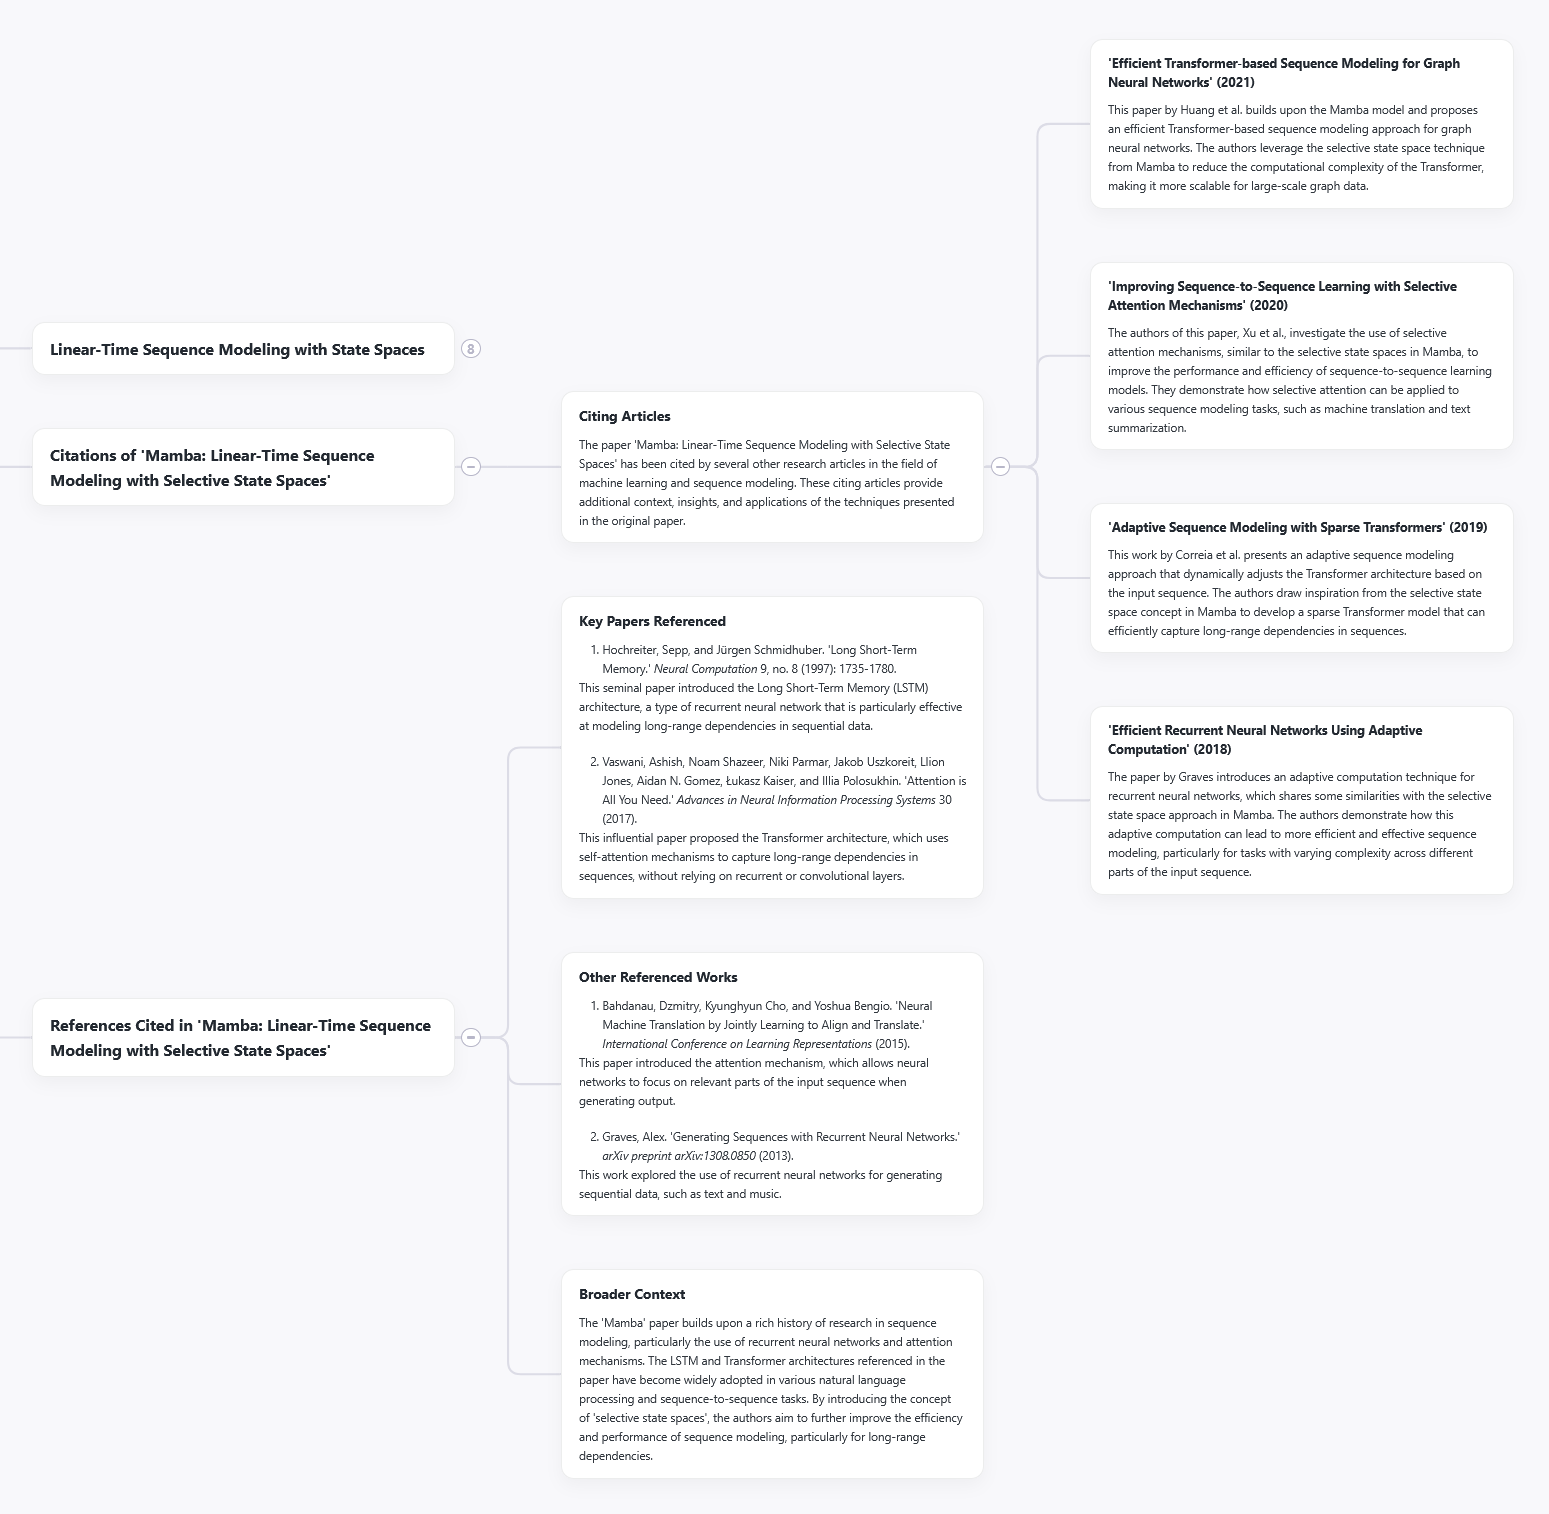
\includegraphics[width=1\textwidth]{cite-network}
\caption{Research Flow中的论文被引和引用关系} 
\label{fig:cite-network}
}

Paper Connect 论文整理助手是另一款强大的AI文献整理工具,能够帮助用户高效地整理和查找学术论文。例如,用户可以请求它在《Nature》子刊上查找最近关于图神经网络方面的文章,如“CGMega: explainable graph neural network framework with attention mechanisms for cancer gene module dissection”,该研究提出了一种基于图注意力机制的深度学习框架,用于癌症基因模块的剖析。此外,它还可以查询《IEEE Transactions on Pattern Analysis and Machine Intelligence》上发表的最新研究,或者在《Journal of Neuroscience》上找到最新的相关文章。对于会议论文,Paper Connect 也能帮助用户查询在 MICCAI 等重要会议上发表的最新成果。通过这些功能,Paper Connect 为研究人员提供了便捷的文献检索服务,节省了大量时间和精力。下面的例子进一步说明了这些。

\prompt{请帮我在Nature子刊上找最近的关于图神经网络方面的文章}

\gpt{
    \textbf{近期研究成果:}
    \begin{itemize}
        \item{GTAT: Empowering Graph Neural Networks with Cross Attention}
        \begin{itemize}
            \item \textbf{期刊}: Scientific Reports
            \item \textbf{发表日期}: 2025年2月8日
            \item \textbf{摘要}: 该研究提出了一种新的图神经网络架构,通过引入交叉注意力机制(Cross Attention)来增强图神经网络的性能。交叉注意力机制能够更好地捕捉节点间的复杂关系,提升模型在图分类和节点分类任务中的表现。
            \item \textbf{链接}: \url{https://www.nature.com/articles/s41598-025-88993-3}
        \end{itemize}
        \item{Graph Geometric Algebra Networks for Graph Representation}
        \begin{itemize}
            \item \textbf{期刊}: Scientific Reports
            \item \textbf{发表日期}: 2025年1月2日
            \item \textbf{摘要}: 该研究探讨了基于几何代数的图神经网络,提出了一种新的图表示学习方法,能够更有效地处理图结构数据。该方法通过几何代数的多维表示,增强了模型对复杂图结构的建模能力。
            \item \textbf{链接}: \url{https://www.nature.com/articles/s41598-024-84483-0}
        \end{itemize}
    \end{itemize}
}